\section{Overview}

\subsection{Introduction}

"Invite Only" is a multi-platform application providing mass access-control to any and all South Africans.

Currently, access-control systems for managing the flow of people into, and out of, a specific space are costly and often require the installation or use of additional hardware like biometric systems, barcode scanners or RFID readers. As a result, mass access-control is a privilege available only to those with the finances to overcome these constraints. The "Invite Only" application aims to change this. With the free download of a single app users will have the power to control and monitor access to any area or event.

The app will allow users to create access-controlled spaces and define constraints for who is permitted to enter these spaces. These constraints may include age restrictions, the amount of people allowed or entrance by invitation only. Then, by scanning identification documents such as South African IDs, driver's licenses or passports, access may be granted or denied on an individual basis - this serves as the primary objective of the application.

Secondarily, creators of access-controlled spaces may allow other user's of "Invite Only" to assist in the access control of these spaces - for example, Jane wants to control access to her party; so, she creates an access-controlled event; however, she would like John to be the person scanning identity documents at the door. Additionally, Jane has constrained the event to only allow entrants who have been invited but she may also want to allow Sarah to invite her group of friends.

Finally, "Invite Only" will give the creators of access-controlled spaces insights into specific metrics. These metrics revolve around who entered, who left and who was inside an access-controlled area at specific times.

With regards to scope, "Invite Only" does not assume the responsibility of keeping unauthorised persons out of any specific area - it merely provides the means to quickly identify whether or not a person is allowed access. Furthermore, "Invite Only" does not ensure that people presenting identification documents are the rightful owners of these documents, this responsibility lies with the user scanning said documents.

\subsection{Domain}
Figure \ref{fig:domain_model} below depicts the domain of the "Invite Only" system. The domain model provides a high-level overview of the context and different role-players involved in the system.

\begin{figure}[H]
  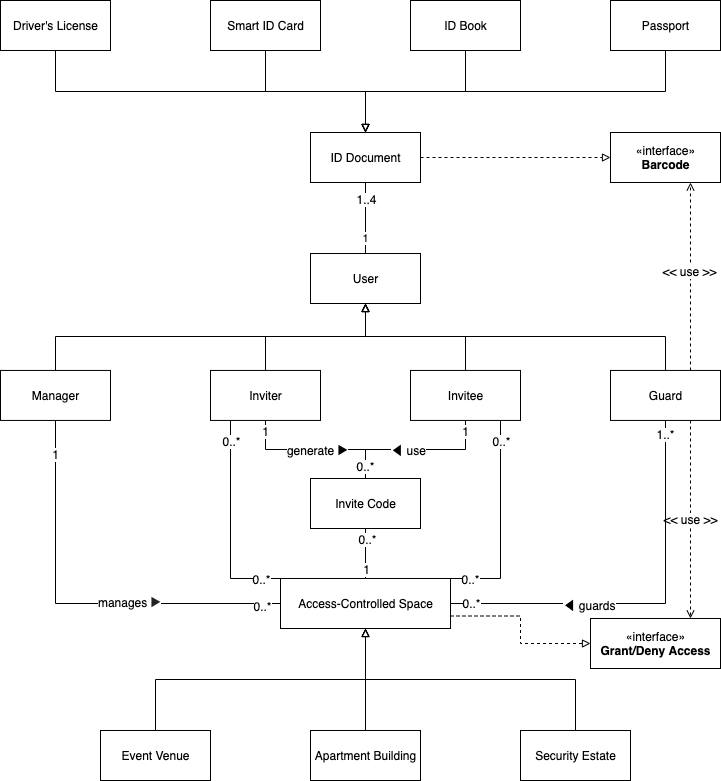
\includegraphics[width=1.0\textwidth]{documentation/software_requirements_specification/overview/domain_model.png}
  \caption{Domain Model}
  \label{fig:domain_model}
\end{figure}

\subsection{User Characteristics}

\subsubsection{Managers}
These include people such as managers of gated communities, apartment buildings, entertainment venues or event-organizers. The intended purpose of these users is to create and manage who is allowed access to spaces as well as grant permissions to other users of "Invite Only" to assist in the access-control of these spaces.

The assumption is that most of these users have attained a level of tertiary education and have some degree of management experience. It is also probable that the users are technically adept with modern mobile operating systems, applications in their management domain and at least some social media platforms, which they would have used for marketing purposes.

Importantly, there will be some user's looking to manage access for one-off occasions. They will have little to no formal education or experience in  management; although, once they have gained access to the "Invite Only" app, the assumption is made that they have at least some experience with modern mobile operating systems and utility applications.

\subsubsection{Guards}
Both doormen and security guards will be using the application to scan people's identification documents and make decisions regarding whether people should be granted access to an access-controlled space.

Formal education is not usually a requirement for these jobs so the assumption is that most of these users have not undergone a great deal of formal education. However, they may still have some experience in the roles they are fulfilling.

Presumably, these users have also worked with identification documents and at least a portion of them with the scanning equipment that is currently circulating in the access-control industry.
\newpage
\subsubsection{Inviters}
This user group consists of residents of gated communities and apartment buildings; or, event VIPs. They will use "Invite Only" to extend invites to access-controlled spaces to their guests. A manager of an access-controlled space is automatically also deemed as an inviter.

Very little is known with regards to who these users are, so their educational and professional backgrounds are impossible to assume. 
Due to the prevalence of existing technologies in the industry, many of these users will be familiar with how current systems work. They will also be familiar with modern mobile operating systems and applications like WhatsApp and Facebook, which are already used excessively by people in these domains.

\subsubsection{Invitees}
Invitees to access-controlled spaces will receive email invites to download and register on "Invite Only". Only after they have registered using an identification document will they be able to enter the access-controlled space using the same document. Managers, guards and inviters of a space are all also deemed as invitees for a that space. 

Again, there is not a great deal that is known with regards to who these users are, so no assumptions are made around their educational or professional backgrounds. 

The one assumption that is made about these users is that they have at least some technical experience because they would have needed a valid email address to register on the app.